\documentclass{article}
\usepackage{blindtext}
\usepackage[a4paper, bottom=1in, top=1in, right=0.75in, left=0.75in]{geometry}
\usepackage{fancyhdr}
\usepackage{minted}
\usepackage[most]{tcolorbox}
\usepackage{graphicx}
\usepackage{tabularx}
\usepackage{array}
% \setlength{\extrarowheight}{15pt}
\definecolor{mygray}{rgb}{0.8,0.8,0.8}
\lstset{%
basicstyle=\ttfamily,
breaklines = true,
backgroundcolor=\color{mygray},
}
\usepackage{realboxes}
\usetikzlibrary{chains,shadows.blur}
\usemintedstyle{lovelace}

\definecolor{lightgray}{rgb}{0.74, 0.74, 0.74}

\DeclareDocumentCommand{\clist}{v}{%
    \Colorbox{mygray}{\csname lstinline\endcsname!#1!}%
}

\begin{document}

\rhead{\thepage}
\lhead{CS201 - Compiler Construction - Zhijia Zhao}

\pagestyle{fancy}

\cfoot{}

% title
\begin{center}

\large{\textbf{Assignment 3}}

\textbf{(Due: Feb 1 23:59)}

Ivan Neto

\end{center}

\vskip 0.2in

\noindent\textbf{Problem 1:} (i) Apply available expression analysis to the following
CFG to find the AvailIn set for each BB ; (ii) Based on the results of available
expression analysis, use GCSE (Global Common Subexpression Elimination) to find out
the redundant computations and remove them.

\newcolumntype{M}[1]{>{\centering\arraybackslash}m{#1}}
\newcolumntype{N}{@{}m{0pt}@{}}

\begin{center}
\includegraphics[scale=0.5]{prob1.png}
\end{center}

\noindent
{\renewcommand{\arraystretch}{2}
\begin{tabularx}{\textwidth}{|X|X|X|X|X|X|}
\hline
Block & A & B & C & D & E \\
\hline
Block & A & B & C & D & E \\ [1em]
\hline
\end{tabularx}
}

\vskip 0.1in

\noindent \textit{Tips: to apply GCSE, you can first find the redundant computations
(expressions), then create the global hash names only for those expressions,
and finally, transform the CFG to remove the redundancies.}


\vskip 0.2in

\noindent \textbf{Solution:}

\vskip 0.1in

\noindent \textbf{Solution 1.1)} Adding version numbers

\vskip 0.2in

% \newcommand*{\yellowemph}[1]{%
% \tikz[baseline]\node[rectangle, fill=green, inner sep=0mm,anchor=base]{#1};%
% }

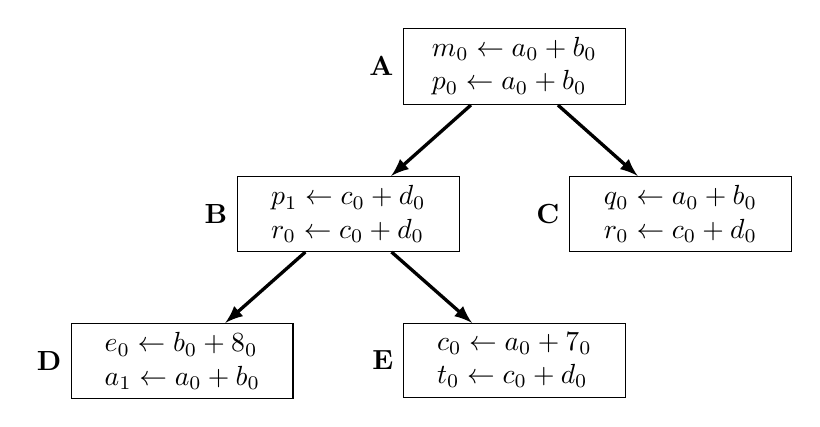
\begin{tikzpicture}[
    node distance = 9mm and 14mm,
    nodestyle/.style = {draw,
                        minimum width=8em,
                        minimum height=2em,
                        align=left,
                        font=\ttfamily},
    arr/.style       = {very thick,
                       -latex}
]
\node (q0) [nodestyle, label=left:\textbf{A}] {
$m_0 \leftarrow a_0 + b_0$ \\
$p_0 \leftarrow a_0 + b_0$
};
\node (q1) [nodestyle, below=of q0, xshift=-6em, label=left:\textbf{B}]    {
$p_1 \leftarrow c_0 + d_0$ \\
$r_0 \leftarrow c_0 + d_0$
};
\node (q2) [nodestyle,below=of q0, xshift=6em, label=left:\textbf{C}] {
$q_0 \leftarrow a_0 + b_0$ \\
$r_0 \leftarrow c_0 + d_0$
};
\draw[arr] (q0) -- (q1);
\draw[arr] (q0) -- (q2);
\node (q3) [nodestyle,below=of q1, xshift=-6em, label=left:\textbf{D}] {
$e_0 \leftarrow b_0 + 8_0$ \\
$a_1 \leftarrow a_0 + b_0$
};
\node (q4) [nodestyle,below=of q1, xshift=6em, label=left:\textbf{E}] {
$c_0 \leftarrow a_0 + 7_0$ \\
$t_0 \leftarrow c_0 + d_0$
};
\draw[arr] (q1) -- (q3);
\draw[arr] (q1) -- (q4);
\end{tikzpicture}

\vskip 0.3in

\noindent \textbf{Solution 1.2)} Adding a hash table status next to each basic block. Also applying Value Numbering.

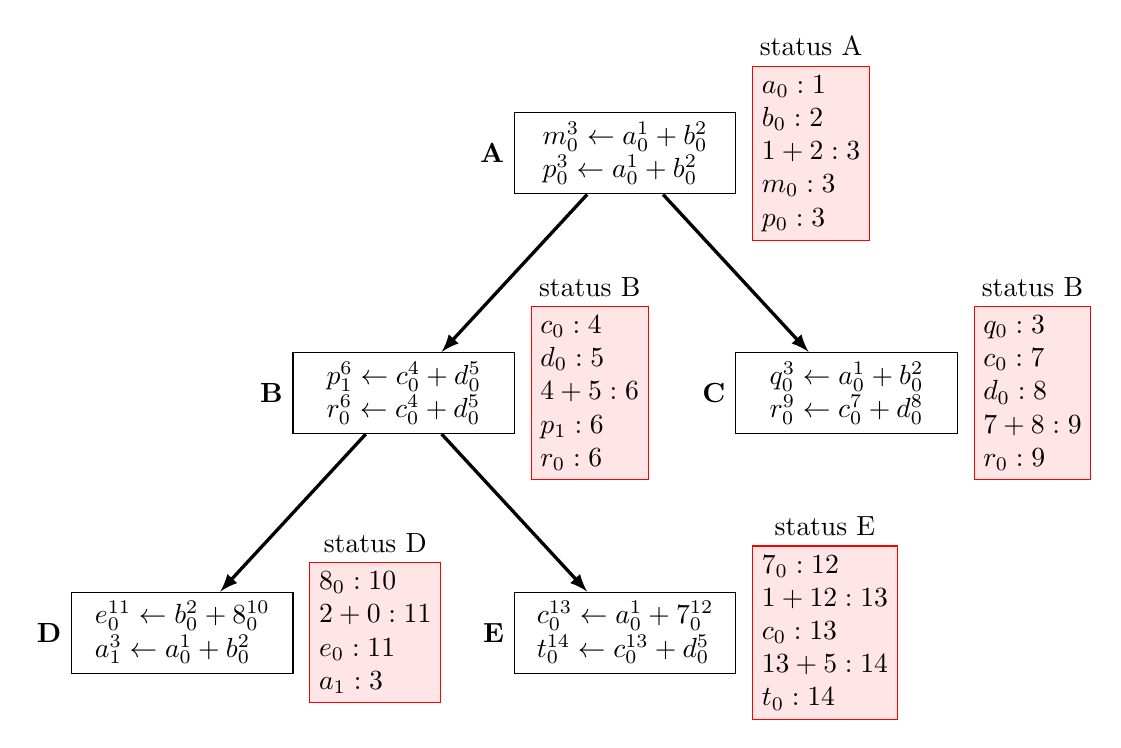
\begin{tikzpicture}[
    node distance = 20mm and 2mm,
    nodestyle/.style = {draw,
                        minimum width=8em,
                        minimum height=2em,
                        align=left,
                        font=\ttfamily},
    hashstyle/.style = {draw=red,
                        fill=red!10,
                        minimum width=4em,
                        minimum height=2em,
                        align=left,
                        font=\ttfamily
                        },
    arr/.style       = {very thick,
                       -latex}
]
\node (q0) [nodestyle, label=left:\textbf{A}] {
$m_0^{3} \leftarrow a_0^{1} + b_0^{2}$ \\
$p_0^{3} \leftarrow a_0^{1} + b_0^{2}$
};

\node (q1) [nodestyle, below=of q0, xshift=-8em, label=left:\textbf{B}]    {
$p_1^{6} \leftarrow c_0^{4} + d_0^{5}$ \\
$r_0^{6} \leftarrow c_0^{4} + d_0^{5}$
};

\node (q2) [nodestyle,below=of q0, xshift=8em, label=left:\textbf{C}] {
$q_0^{3} \leftarrow a_0^{1} + b_0^{2}$ \\
$r_0^{9} \leftarrow c_0^{7} + d_0^{8}$
};

\node (q3) [nodestyle,below=of q1, xshift=-8em, label=left:\textbf{D}] {
$e_0^{11} \leftarrow b_0^{2} + 8_0^{10}$ \\
$a_1^{3} \leftarrow a_0^{1} + b_0^{2}$
};

\node (q4) [nodestyle,below=of q1, xshift=8em, label=left:\textbf{E}] {
$c_0^{13} \leftarrow a_0^{1} + 7_0^{12}$ \\
$t_0^{14} \leftarrow c_0^{13} + d_0^{5}$
};

\draw[arr] (q0) -- (q1);
\draw[arr] (q0) -- (q2);
\draw[arr] (q1) -- (q3);
\draw[arr] (q1) -- (q4);

\node (h0) [hashstyle, label=above:status A, right=of q0] {
    $a_0: 1$ \\
    $b_0: 2$ \\
    $1+2: 3$ \\
    $m_0: 3$ \\
    $p_0: 3$
};
\node (h1) [hashstyle, label=above:status B, right=of q1] {
    $c_0: 4$ \\
    $d_0: 5$ \\
    $4+5: 6$ \\
    $p_1: 6$ \\
    $r_0: 6$
};
\node (h2) [hashstyle, label=above:status B, right=of q2] {
    $q_0: 3$ \\
    $c_0: 7$ \\
    $d_0: 8$ \\
    $7+8: 9$ \\
    $r_0: 9$
};
\node (h3) [hashstyle, label=above:status D, right=of q3] {
    $8_0: 10$ \\
    $2+0: 11$ \\
    $e_0: 11$ \\
    $a_1: 3$
};
\node (h4) [hashstyle, label=above:status E, right=of q4] {
    $7_0: 12$ \\
    $1+12: 13$ \\
    $c_0: 13$ \\
    $13+5: 14$ \\
    $t_0: 14$
};

\end{tikzpicture}

\vskip 0.3in

\noindent \textbf{Solution 1.3)} Writing down transformed EBB after removing redundancies

\vskip 0.2in

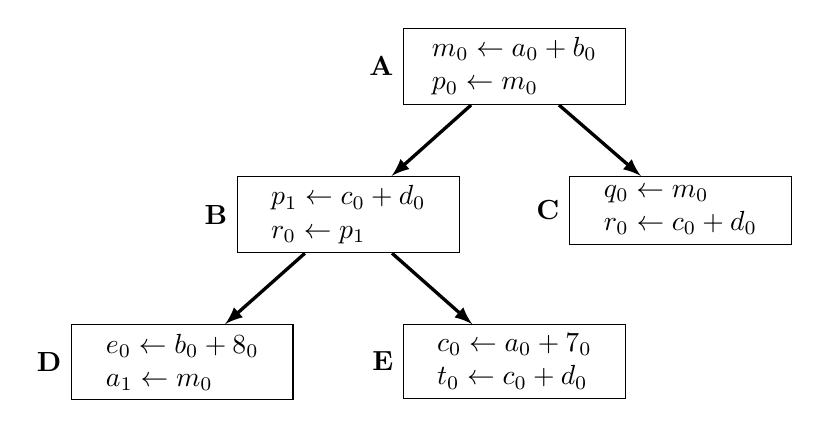
\begin{tikzpicture} [
    node distance = 9mm and 14mm,
    nodestyle/.style = {draw,
                        minimum width=8em,
                        minimum height=2em,
                        align=left,
                        font=\ttfamily},
    arr/.style       = {very thick,
                       -latex}
]
\node (q0) [nodestyle, label=left:\textbf{A}] {
$m_0 \leftarrow a_0 + b_0$ \\
$p_0 \leftarrow m_0$
};
\node (q1) [nodestyle, below=of q0, xshift=-6em, label=left:\textbf{B}]    {
$p_1 \leftarrow c_0 + d_0$ \\
$r_0 \leftarrow p_1$
};
\node (q2) [nodestyle,below=of q0, xshift=6em, label=left:\textbf{C}] {
$q_0 \leftarrow m_0$ \\
$r_0 \leftarrow c_0 + d_0$
};
\draw[arr] (q0) -- (q1);
\draw[arr] (q0) -- (q2);
\node (q3) [nodestyle,below=of q1, xshift=-6em, label=left:\textbf{D}] {
$e_0 \leftarrow b_0 + 8_0$ \\
$a_1 \leftarrow m_0$
};
\node (q4) [nodestyle,below=of q1, xshift=6em, label=left:\textbf{E}] {
$c_0 \leftarrow a_0 + 7_0$ \\
$t_0 \leftarrow c_0 + d_0$
};
\draw[arr] (q1) -- (q3);
\draw[arr] (q1) -- (q4);
\end{tikzpicture} 

\end{document}
